\documentclass[twoside,a4]{report}
\def\atitle{Development of a Rheometer Controller Using a Raspberry Pi}
\def\shorttitle{Development of a Rheometer Controller}
\def\theauthor{Christopher Boyle}
\def\thewords{5087} % last proper build on Wed 08 March 2017 at 17:57:59

\def\br{\newline \newline \noindent}
\def\hi{\huge{!!!}}
\def\nohi{!!!! \normalsize}
\def\cbh{\large\bfseries !!! ??? !!! \normalsize\normalfont}

% Imports
\usepackage{graphicx}
\usepackage[a4paper]{geometry}
\usepackage{fancyhdr}
\usepackage[english]{babel}
\usepackage{etoolbox}
\usepackage{url}
\usepackage[hidelinks]{hyperref}
\usepackage{subcaption}

% Unused packages
%\usepackage{placeins}
%\usepackage{fancyref}
%\usepackage[comma,authoryear]{natbib}
%\usepackage{lipsum}

% Settings
\geometry{top=2cm, bottom=2.5cm, left=3cm, right=2.5cm}  % Sets the mnargins

%\patchcmd{\chapter}{\thispagestyle{plain}}{\thispagestyle{plain}}{}{}  % not sure?
%\patchcmd{\section}{\thispagestyle{plain}}{\thispagestyle{plain}}{}{}
%\patchcmd{\subsection}{\thispagestyle{plain}}{\thispagestyle{plain}}{}{}

\setcounter{secnumdepth}{0}  % removes the numbering from toc entires

%\renewcommand{\theequation}{\arabic{equation}}  % not sure?

\renewcommand\UrlFont{\rmfamily\itshape}  % sets URL font to normal font (rather than code font)

\setlength{\fboxsep}{0pt}  % separator length around figure boxes
\setlength{\fboxrule}{0pt}  % rule width around figures

\def\achapter{preamble}  % set the command "achapter" to  the name of the current section
\def\rpilong{Raspberry Pi}
\def\rpi{\(R\pi\)}
%=====------++++++=====------++++++=====------++++++=====------++++++=====------++++++=====------++++++=====------++++++=====------++++++=====------++++++=====------++++++=====------++++++=====------++++++=====------++++++=====------++++++=====------++++++=====------++++++
% TEMPLATES

\iffalse  % This bit won't go onto the PDF


%%%EQUATION

	\begin{equation}
		(THE EQUATION)
		\label{EQUATION REF}
	\end{equation}


%%%FIGURE

	\begin{figure}[!htb]
		\centering
		\fbox{\includegraphics[scale=SCALE]{IMAGE LOCATION}}
		\caption{CAPTION}
		\label{FIGURE REF}
	\end{figure} \newline  \noindent

%%%BULLET POINT LIST
	\begin{itemize}
	\item
	\end{itemize}

\fi

%=====------++++++=====------++++++=====------++++++=====------++++++=====------++++++=====------++++++=====------++++++=====------++++++=====------++++++=====------++++++=====------++++++=====------++++++=====------++++++=====------++++++=====------++++++=====------++++++

% Header/footer preamble
\fancyhf{}  % clear the current header footer
\fancypagestyle{plain}{  % add settings for plain page style
	\renewcommand{\headrulewidth}{0.4pt}  % weight of the header rule (set to 0 for no line)
	\renewcommand{\footrulewidth}{0.4pt}  % height of the footer rule (set to 0 for no line)
%	\fancyhead[L]{\atitle}  % Header left is title
	\fancyhead[LE]{\achapter}  % Header left is name of chapter
	\fancyhead[RO]{\shorttitle}  % Header left is name of chapter
	\fancyhead[RE,LO]{\theauthor}  % Header right is author name
	\fancyfoot[LO,RE]{\today}  % Footer left is date
	\fancyfoot[RO,LE]{\thepage}  % Footer right is page number
}
\pagestyle{plain}

\begin{document}
%%%%%%%%%%%%%%%%%%%%%%%%%% TITLE PAGE
	\begin{titlepage}
		\makebox[\textwidth][c]{
\includegraphics[scale=1]{images/titleheader.png}}
		\centering
		\vskip3cm
		{
			\bfseries\Large
			Department of Chemical \& Process Engineering\\
			\vskip1cm
			MEng in Chemical \& Process Engineering\\
			18530
			\vskip3cm
			\LARGE\atitle
		}
		\vskip3cm
		{\small Word Count: \thewords}
		\vskip1cm
		\begin{flushleft}
			This project is submitted in partial fulfilment of the regulations governing the award of \\
			Degree of MEng in Chemical Engineering at the University of Strathclyde
			\vskip2cm
			Your name: Christopher Boyle \hfill Date: \today
			\vskip1cm
			Organisation: University of Strathclyde, Department of Chemical \& Process Engineering\newline% \newline
			In-house Supervisor: Dr. Leo Lue \newline% \newline
			Academic Supervisor: Dr. Leo Lue
		\end{flushleft}
	\end{titlepage}

	%%%%%%%%%%%%%%%%%%% Main Content Settings
	\pagenumbering{roman}
	
	%%%%%%%%%%%%%%%%%%%%%%%%%%%%%%%%%%%%%%%%%% MAIN BODY PREAMBLE
	% Summary Page
	\chapter*{Summary}
	\addcontentsline{toc}{chapter}{Summary}
	\def\achapter{Summary}
	%Brief, factual, generally following the same order of presentation as the report. Do not include figures, tables, or references.
	\newpage
	
	% Contents Page
	\def\achapter{Contents}
	\tableofcontents
	
	% Acknowledgements
	\chapter*{Acknowledgements}
	\addcontentsline{toc}{chapter}{Acknowledgements}
	\def\achapter{Acknowledgements}
	%It is a matter of honesty and courtesy that acknowledgement is made to those who helped you in your work.
	%Dr. Lue
	%Jim Murphy
	%Aditi Mukhopadhyay
	%Stack Exchanger Electrical Engineering Community
	
	\newpage
	\pagenumbering{arabic}
	\setcounter{page}{1}
	
%=====------++++++=====------++++++=====------++++++=====------++++++=====------++++++=====------++++++=====------++++++=====------++++++=====------++++++=====------++++++=====------++++++=====------++++++=====------++++++=====------++++++=====------++++++=====------++++++
                                                               
	\chapter*{Introduction}
	\addcontentsline{toc}{chapter}{Introduction}
	\def\achapter{Introduction}
	%The introduction sets the scene. It should include a brief description of the organisation, the type of work carried out, projects undertaken, background information to the work carried out and a brief outline of the report and of the learning objectives for the project.
	%History of what is being done, what is used to do it, how it is done.



	\section{Laboratory Automation and Process Control} % section last edited 3/3/2017
	Laboratory automation involves the design and implementation of robotic systems which are able to conduct laboratory experiments automatically, reducing the workload of human scientists and technicians \cite{backwhatisauto}. This includes the use of machine learning and AI to interpret results and create hypotheses \cite{backlitrevai, backbaconauto, backlabauto}. The motivation for this is eaasy to see, "Robot Scientists" can be used to conduct experiments with little to no human supervision and can take in a vast number of measurements. The "Adam" Robot Scientist developed by the team at Aberystwyth University can make over 1,000,000 observations and hypotheses per day \cite{backontorobsci}. \br
	Laboratory automation emerged in the late 19th century, with siphons and controlled flow of water used to automate various processes. As technology advanced and electronics became more prevalent, the options for automation in the laboratory increased. Automatic titration equipment (using photo-cells to detect a colour change) were revolutionary in their ability to accurately and consistently record results, especially for difficult to discern colour changes \cite{backlabautohisto}. \br
	Process control is a form of laboratory automation, using technology to replace the need for manual intervention in the running of a process. Process control has developed along a similar path to laboratory automation; starting with mechanical analogue devices, then moving into electronically assisted technology and then, with the advent of computer technology, process control became what it is today \cite{backautocontrolhisto}.
	%Laboratory automation is similar in concept to process control, both using computers to manage the running of a process. %? How else to word this...
	Process control is an inherent area of process design; the process (whatever it may be) has parameters which must be controlled so that the process continues under the design paramters; at the correct temperature, pressure, etc. Process control has historically been achieved through the use of analogue equipment, using pressurised air to send and receive signals from process equipment. Modern process control is achieved through the use of computers and digital electronics, where the analogue measured signals are converted into digital signals, so that a computer can understand the data. The controller applies an algorithm to calculate the control action required to maintain the desired value of the variable. The modern digital controller can deal with almost any form of input, guarding against a wide variety of disturbances. If it can be measured, it can be controlled.\br
	At the heart of the modern controller is the control algorithm. This is the calculation which determines what change to the control output needs to be made (the control action). Control algorithms vary with application. The most commonly used algorithm is the Proportional-Integral-Derivative algorithm (PID control), consisting of three sections which can be turned off or on depending on the needs of the situation:
	\begin{itemize}
	\item Proportional control increases the control action proportional to the size of the error (the difference between the set point and the measured value). This is easy to tune and set up, however it suffers from offset bias. This bias arise from the control action being balanced out in the process by the error such that the control action is not sufficient to change the process to compensate for the error. The error will remain, and the controller will do no more to correct for it, thus an offset is sustained. This must be manually corrected for.
	\item Integral control increases the control action depending on the integral of the error with respect to time (the longer the error goes on, the higher the control action). Integral action is useful to eliminate the offset bias of proportional control.
	\item Finally, derivative control increases control action with the derivative of the error with respect to time, so a quickly rising error is met with a large change in control action. Derivative action is difficult to tune and highly sensitive to noise in the circuit - this means it is rarely used. If it is used, it requires some form of noise filter on the signal and careful tuning. The most common version of the PID algorithm only uses proportional and integral action (no derivative) - the PI controller. PI control allows for easy tuning and quick response, without the difficulties of derivative action, or the offset bias of proportional control.
	\end{itemize}
	Each control element has an associated gain parameter which affects how strongly that element is represented in the control action. These parameters must be set properly before controller can be used. This is done in a process called tuning. There are a variety of methods for tuning the controller, most commonly used is the Ziegler-Nichols method, involving tuning the controller such that the measured value oscillates in a sustained way. Then using the period of oscillation along with other measured parameters to decide on the optimum controller tuning. After tuning using a method such as Ziegler-Nichols it is often required to tweak the tuning manually to obtain the most effective controller for the situation. This is done mostly by trial and error. Trial and error tuning can also be used to fully tune the device, although this would take a long time to do by hand. \br
	The controller device itself is a small computer, reading input from the instruments and then applying the algorithm to determine how it should alter the process. These small computers are called "microcontrollers". A microcontroller chip is a small re-programmable computer which reads input from, and outputs data to an electronic circuit \cite{backwhatismc}. Microcontrollers are programmed by connecting them to a "master" computer which can set the data on the microcontroller's storage. Data is stored as binary data (data is stored solely in the form of 0s and 1s). The program is written in a programming language, a special set of instructions which the environment can understand and convert into actions. \br
	
%	\begin{figure}[h!]
%	\centering
%	\fbox{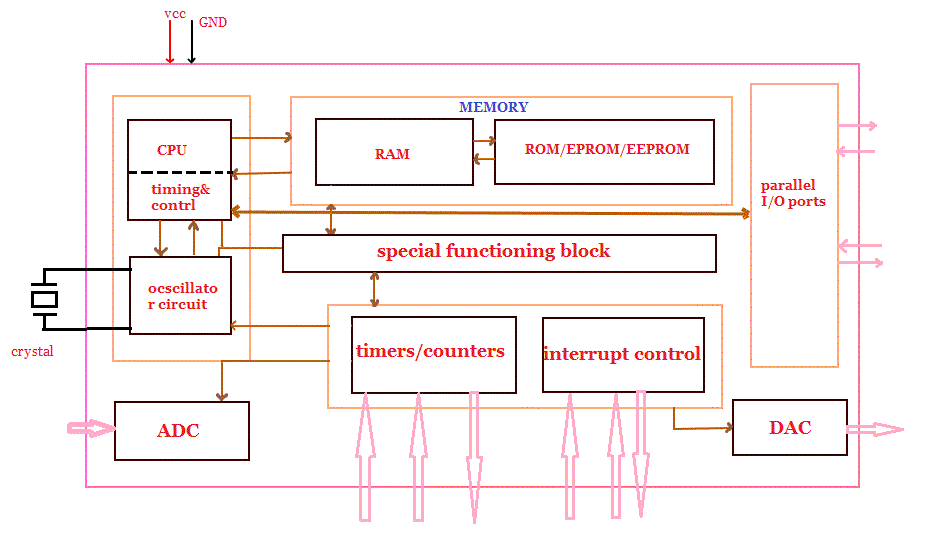
\includegraphics[scale=0.5]{images/mcudia.png}}	\caption{Microcontroller Block Diagram (taken from  \cite{mcudia})}
%	\label{mcudia}
%	\end{figure}

	


	\section{Raspberry Pi} % section last edited 3/3/2017
	\noindent
	Microcontrollers are commonly used in education to teach computer programming \cite{backmcedu1, backmcedu2}. However, it was noticed that people were not properly learning about how computers work in schools and universities and so a team of academics at the University of Cambridge created the Raspberry Pi Foundation, and developed the Raspberry Pi Model A as a platform to facilitate education \cite{pihistory}. The Raspberry Pi is a small (85mm x 56mm \cite{pi3mechdraw}) computer. By default, it runs a version of GNU/Linux called "Raspian". There are a number of alternative operating systems suitable for different applications (media center, embedded smart technology) \cite{piotheros}.  \newline
	\begin{figure}[!htb]
	\centering
	\fbox{\includegraphics[scale=0.3]{images/annotpidia.png}} %https://www.draw.io/#Hcbosoft%2Fpi_rheo_proj%2Fmaster%2Fwrite_up%2Fimages%2Fannot_pi_dia.xml
	\caption{Raspberry Pi 3 Model B (taken from  \cite{pi3info})}
	\label{pidia}
%	\footnotesize Clockwise from top left: GPIO pins, USB ports, Ethernet port, audio jack, Camera Serial Interface (CSI), HDMI port, micro-USB power port, and Display Serial Interface (DSI).
	\end{figure} \newline% \noindent
	The first Raspberry Pi (Model A) had a single core 700MHz processor and 256MB of RAM \cite{pi1info}, while the current Raspberry Pi 3 Model B has a quad core 1.2GHz and 1GB of RAM (also including built in WiFi and Bluetooth) \cite{pi3info}. The quad core processor enables better multi-threaded operation for software running on the Raspberry Pi, meaning that big cumbersome programs can run much more efficiently than before. In addition, the increase in memory and CPU clock frequency means there is overall a massive performance boost. Operations like compiling a large program (for example OpenCV, the Open Source Computer Vision Library) which could take over 9 hours \cite{pipowercompold} on the Raspberry Pi 1, takes little over an hour and a half \cite{pipowercompnew} on the latest model.\br
	Despite being initially designed for educational purposes, the Raspberry Pi has found success in other areas such as with hobbyists \cite{pihobbynotedu} and in industry \cite{pimorethanedu}. What makes the Raspberry Pi attractive as a process controller are the GPIO pins (General Purpose Input/Output, see Figure \ref{pidia}) made available on the main board, similar to a microcontroller. These pins allow electronic circuits to interface with the Raspberry Pi, and thus software to interact with the real world in a way that is not easy to accomplish with a traditional computer. This marriage of microcontroller and desktop computer allows for development, and testing in a single package. In addition, the Raspberry Pi retails (at the time of writing) for \pounds 30.00 \cite{picost}, making it a very cost effective alternative to other control solutions (which can cost several hundred pounds \cite{otherpcucost}). \br
	The GPIO pins are the heart of the Raspberry Pi. Each pin is numbered so that they can be referenced and distinguished between their functions. Some of the pins on the GPIO header are power pins (e.g.  pins 1,2 and 4), some are ground (e.g. 6, 9, and 14), and most are GPIO pins (e.g. 3, 5, and 7). Each GPIO pin can be either low or high. This can be set in different ways; resistors attached to the GPIO pins can be used to "pull-up" or "pull-down" the signal. If a pin is pulled down, its signal is normally low - it needs to be actively raised high. If a signal is pulled up, it is normally high - it can be lowered by connecting it to ground, but without that it will try to be high. These pull-up and pull-down resistors are included in the Raspberry Pi internally and can be turned on or off via software. \newline
	\begin{figure}[!htb]
	\centering
	\fbox{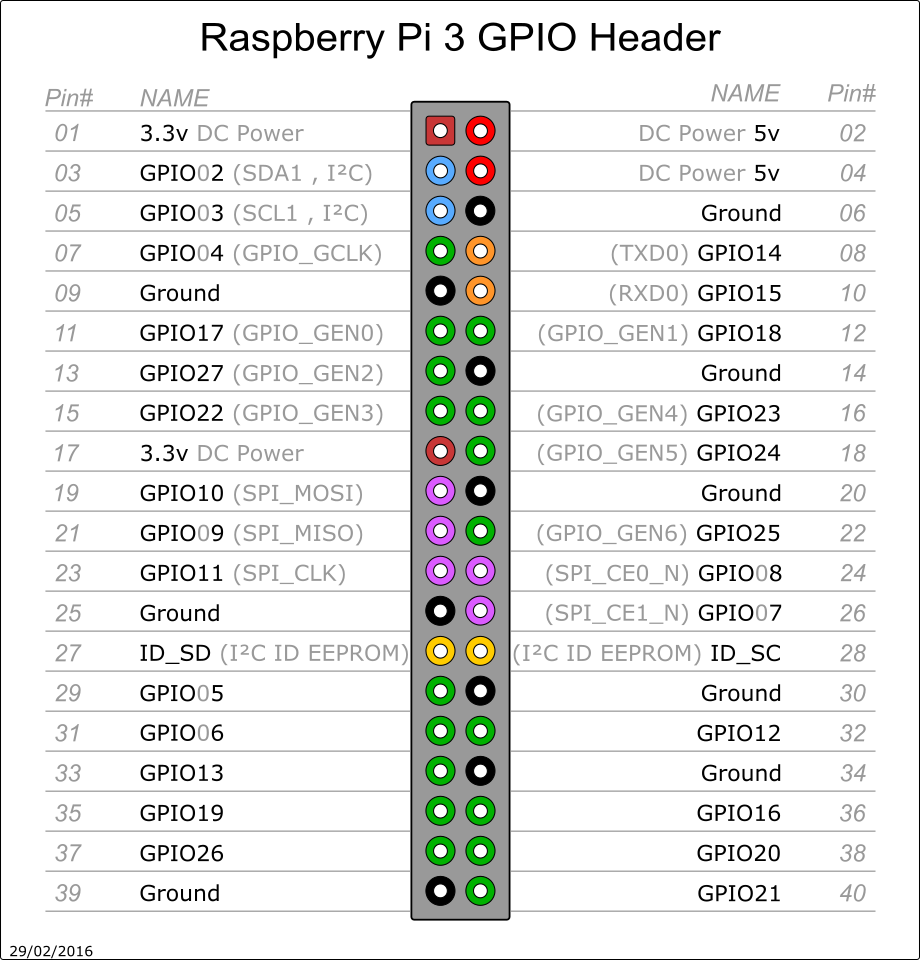
\includegraphics[scale=0.2]{images/gpiopinout.png}}
	\caption{Raspberry Pi 3 Model B GPIO Pinout Diagram (taken from  \cite{pigpiopinout})}
	\label{gpiopinout}
	\end{figure} \newline  \noindent
	In addition to simple GPIO functionality, some of the Raspberry Pi's GPIO pins have special functionality, like the ability to use serial communication making inter-device communication much easier. To send the number 1750 to an integrated circuit, the Raspberry Pi would need at least 11 free GPIO pins. While this is not impossible, the number of GPIO pins taken up by the single device is extremely inconvenient. This can easily be sent via serial connection with just two wires. Pins 3 and 5 can also be used to communicate with integrated circuits with the \(I^2 C\) protocol (Inter-Integrated Circuit). This allows bytes of data to be sent over only two wires \cite{backwhatisi2c}. This is done by \textit{serial communication}. Serial communication is where each bit of data (starting with the most significant bit, the highest value bit) is sent one after the other down a wire (the "data" line) \cite{backwhatisserpar} while another wire is used to synchronise the communication beteween devices (the "clock" line). Pins 19, 21, 23, 24, and 26 are used for another serial communications protocol, the Serial Peripherial Interface (SPI) protocol \cite{backwhatisspi}. SPI is similar to \(I^2 C\), although it differs in a few key ways.  \(I^2 C\) manages sub devices on the network using an address system which enables anything up to 128 devices connected together in one go, however SPI uses a simple select system where a signal is sent from a GPIO to the SPI device to tell it to expect instruction. This makes the SPI device far easier to work with, but less useful as the number of daisy-chained devices is limited by the number of free GPIO pins. \br
	The high level languages used to create programs on desktop computers can be similarly used to write software on the Raspberry Pi. There are a number of software packages available for facilitating the communication with the GPIO pins. Built in to the Raspberry Pi are some basic packages, but for greater functionality third-party libraries are available for anyone to download and use\cite{pilibswiringpi, pilibspigpio}. The programming language "Python" is popular among software developers. Python is a high level, object oriented, interpreted language; making it well suited to quickly develop clean and easy to use software. Due to its popularity, Python has a vast number of packages available to perform any number of functions.
	
	\section{Rheometry} % last edited 8/3/2017
	The viscosity of a fluid is a measure of how resistant it is to flow. This is an important concept in process engineering: most processes involve fluids, many products are have fluid components. The viscosity (\(\mu\)) of a fluid can be calculated from the shear stress (\(\tau\)) imposed on a fluid and the rate at which it shears(\(\dot{\gamma}\)) using Newton's Law of Viscosity (Equation \ref{eqnvisco}) \cite{backfluidmech}.
	\begin{equation}
	\mu = \frac{\tau}{\dot{\gamma}}
	\label{eqnvisco}
	\end{equation}
	There are different classes of fluids depending on how their viscosity behaves with respect to shear rate (the speed of the deformation) or the shear stress (the force behind the deformation). Newtonian fluids (like water) have a viscosity which is independent of the shear stress - proportional only to the shear rate. Some fluids have time-dependant viscosities: thixotropic fluids have a viscosity which apparently reduces the longer a stress is applied, and rheopectic fluids have a viscosity which apparently increases the longer a stress is applied. Other non-Newtonian fluids are dependant on the magnitude of the stress: shear-thinning fluids have a viscosity that appears to decrease with increased stress, and shear thickening fluids appear to experience a viscosity increase with an increase in stress \cite{backtypesofnonnewt}. Figures \ref{figshearthin} \& \ref{figshearthick} give examples of how shear rate varies with shear stress for non-Newtonian fluids. \br
	\begin{figure}[!htb]
		\centering
		\fbox{
			\begin{subfigure}[t]{0.45\textwidth}
				\centering
				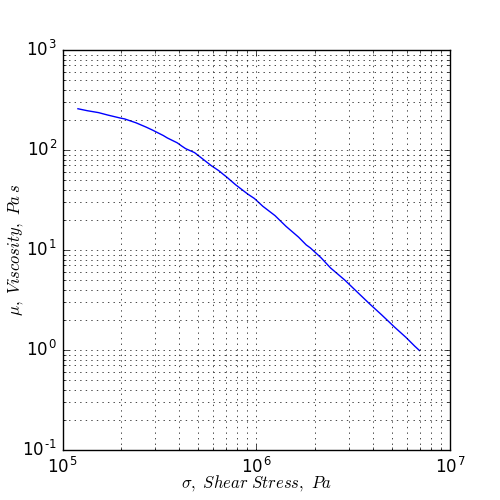
\includegraphics[scale=0.5]{figures/fig_shear_behav_thin.png}
				\caption{Shear Thinning}
				\label{figshearthin}
			\end{subfigure}
			\begin{subfigure}[t]{0.45\textwidth}
				\centering
				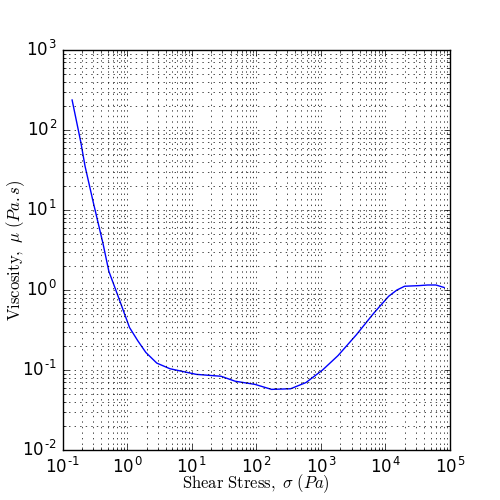
\includegraphics[scale=0.5]{figures/fig_shear_behav_thick.png}
				\caption{Shear Thickening}
				\label{figshearthick}
			\end{subfigure}
			%\fbox{\includegraphics[scale=0.25]{figures/fig_shear_behav.png}}
		}
		\label{figshearthinthick}
		\caption{Non-Newtonian Behaviour: Viscosity vs Shear Stress (adapted from \cite{figshearthin, figshearthick})}
	\end{figure} \newline  \noindent
	Viscosity is measured in the lab using a rheometer. There are several distinct types of rheometers: capillary rheometers flow the fluid through a pipe of known dimensions and use the time taken to calculate the viscosity, cone-and-plate rheomters use a plate upon which is the fluid to be tested, and into the fluid is placed a cone which is spun (using the geometry and the torque/rotational rate of the spinning cone to calulate the viscosity), and the rotational rheometer which consists of a cylinder within another with the fluid to be tested between the cylinders such that it shears when a cylinder is rotated. \br
	The capillary rheometer consists of a tube of known cross section, through which the test fluid is forced (by pumping, by piston). The viscosity can be found by measuring the flow rate and pressure gradient, and using the Hagen-Poiseulle equation for laminar flow through a pipe \cite{backcaprheom}. \cbh \br %(Information about the CR: how accurate can it be, what is it usually used for)
	The cone-and-plate rheometer \cbh \br %(Information about the CAPR: how does it work, how accurate can it be, what is it usually used for)
	The rotational rheometer is based upon the idea of couette flow: two infinitely long plates (separated by a known amount) between which is the fluid. In this scenario, \cbh
	constructed from two cylinders: the outer (hollow) cylinder and the inner cylinder. The cylinders are positioned vertically close together to limit the amount of fluid shearing on the bottom of the inner cylinder.
	
	\section{Colloidal Suspensions and Jamming} % last edited 8/3/2017
	Fluids consisting of solid particles suspended in a liquid are prone to non-Newtonian behaviour, most commonly shear thinning (pseudoplastic). Some suspensions exhibit shear thickening behaviour, which has been explained in a number of ways. The hydroclustering theory is that with increased shear stress, the particles stick together more, causing an apparent increase in viscosity. \cbh %more info.
	The order-disorder transition  theory explains the increase in viscosity as being due to an increase in stress causing the particles to become disordered. Initially there is a drop in viscosity, due to the particles in the suspension becoming more ordered. Then, as the stress is increased past a yield stress, the viscosity begins to increase due to a disruption in the order of the particles. % other theories?
	\cbh \br
	Shear thickening can be split further into continuous shear thickening (CST) and discontinuous shear thickening (DST, also termed dilatancy). CST is where the viscosity increases proportionally past a yield stress. However, with DST the viscosity suddenly (almost asymptotically) jumps upwards after a yield stress. DST has been associated with an apparent decrease in volume fraction of suspensions - hence its alternative name of dilatency. This effect also lends credence to the order-disorder-transition theory of shear thickening: you would expect the volume fraction to decrease (void fraction to increase) if the particles are going from a neat, ordered arrangement into extreme disorder. \cbh \br % cite!
	Jamming, problems \cbh \br
	\textit{"the conversion of a liquid system into a solid by imposed stress"} \cite{backhawjam} \cbh \br
	void fraction \cbh \br
	\( \Phi = 0.64 \) \cite{backguypoonjam} \cbh \br
	void frac v jamming probability \cbh \br
	hard spheres \cbh \br
	
	"Normal" fluids (like water) exhibit Newtonian behaviour, this means that the rate of shear (how fast they deform) is directly proportional to the shear stress imposed upon them, with the constant of proportionality being the viscosity of the fluid\cite[p.~252]{schadict}. Multiphase suspensions can exhibit non-Newtonian viscous behaviour, where this direct relationship is not found \cite[p.~255-256]{schadict}. Some exhibit a shear-thickening behaviour: as the shear stress is increased, the shear rate decreases faster than in newtonian behaviour and others exhibit shear thinning .  Continuous shear thickening (shown in Figure \ref{figshearthick})  is an increase in the apparent viscosity. Discontinuous shear thickening is a sudden and extreme increase in the apparent viscosity of the fluid and is closely related to jamming, which is \textit{"the conversion of a liquid system into a solid by imposed stress"} \cite{backhawjam}. Jamming is found in many different systems: in solids entering a hopper \cite{back2djam}, in pedestrians walking down a corridor \cite{backpedjam}, and in traffic \cite{backcarjam}. This can cause problems in processes: halting flow, damaging mixing equipment \cite{backshearjambertrand}. \br
	Volume fraction of the suspension mixture is an important property when looking at jamming. A suspension's volume fraction (\( \Phi \)) is the ratio of the volume of suspended particles to the volume of fluid in the suspension. For spherical particles, there is a maximum fraction. The closest packing that can occur (face-centred cubic) results in a particle volume fraction of \( \Phi = 0.74 \). However, at this packing the suspension is no longer a suspension and the particles are all in constant contact. The highest volume fraction of a suspension that still allows fluid to pass between the particles (particles are lubricated) is \( \Phi = 0.64 \) \cite{backguypoonjam}. As volume fraction increases, the likelihood of a suspension to undergo jamming increases (CITE).
	
	%flow, shear, jam frequency %TODO
	An interesting phenomenon that occurs in shearing suspensions is the formation and dissipation of "cracks" on the surface of the suspension. This can be directly seen in Figure \ref{cforscracks}. The cracks have been associated with a localized change in volume faction of the suspended particles \cite{backhawjam}. Another interesting optical property of jammed suspensions: the surface of a shear suspension has been found to alter texture, evidence of "Dilation" \cite{backbrownjaegrev}: caused by the particles in shear attempting to move around each other but having to take an inefficient route therefore decreasing the volume fraction of the suspension. This draws more fluid into the bulk and then the surface appears rough in texture, as opposed to glossy. 
	\newline \newline \noindent
	\begin{figure}[!htb]
		\centering
		\fbox{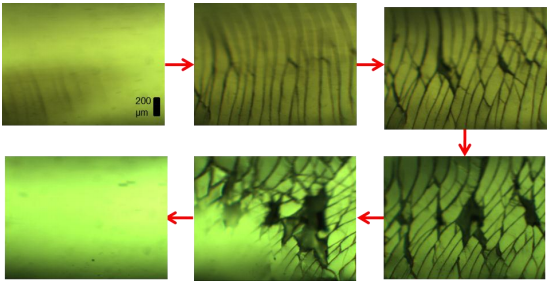
\includegraphics[scale=0.4]{images/cfors_cracks.png}}
		\caption{Suspension Surface Cracks (taken from \cite[p.~118]{thescforsyth})}
		\label{cforscracks}
	\end{figure} \newline  \noindent
	

	\section{This Project} % last edited 3/3/2017
	This project aims to design, build, and test a control system for a bespoke jamming-focussed experimental rheometer. The experiment itself aims to gather more information about the statistical probability of the occurrence of a jam and how the shear stress affects this. \br
	The experimental process consists of two concentric cylinders, the inner of which is attached to a DC motor and can be rotated. The gap between the two cylinders will be filled with a colloidal suspension. As the inner cylinder is rotated, the suspension will be subject to either a constant shear force, or a constant shear rate. 
	%To find out how the formation of the cracks on the fluid's surface during shear correlate with the occurrence of discontinuous shear thickening, a camera will be aimed at the surface of the shearing fluid throughout the course of the experiment. The camera will be optically magnified using lenses placed in front of the aperture and will record images, which can later be processed using image recognition software to detect the formation of the cracks. \newline \newline \noindent
	By knowing the power sent to the motor, as well as its efficiency and rotational speed, the strain rate and stress imposed upon the fluid in the rheomter can be calculated and thus used to obtain the rheology of the fluid - how the viscosity varies with time and stress. \br
	The experimental set-up will be controlled by a Raspberry Pi 3 Model B. The Raspberry Pi's low cost, low power consumption, and GPIO availability make it a suitable choice for the controller to this process. Software will be developed for the Raspberry Pi to read in the motor's speed and the PEND's voltage reading, record it accurately and to control the rotational speed of the motor. In addition, the Raspberry Pi can be used to automate the experimental process by automatically altering experimental parameters in-between runs while logging all the relevant data during runs. The Pi can also be set up with a web interface, allowing monitoring of the experiment from remote locations, further reducing the manual workload on lab technicians. \br
	Hardware was be developed to allow the Raspberry Pi to obtain the most accurate readings from the experiment as possible; the rotational speed of the motor, the electrical power supplied to the motor, the current shear stress observed within the fluid, and the presence of 'cracks' on the surface of the fluid.\br
	Software will be developed to facilitate the accurate reading of information from the experiment, as well as control of the experimental parameters. There are two general operating modes; constant shear rate (or rotational speed), and constant shear stress (or torque). The former is relatively simple to do. By recording the motor's rotational speed and comparing with a set point, the speed can easily be held at a fixed point (thus a constant shear rate is achieved). The output torque is fixed in a similar way, using feedback from the process to fix the torque from the motor.

	%\chapter*{Description of the Organisation} % last edited 3/3/2017
	%\addcontentsline{toc}{chapter}{Description of the Organisation}
	%\label{chap:doo}
	%\def\achapter{Description of the Organisation}
	%In this section, you should show a good understanding of the organisation. Details may include the type of organisation, management structure, products, and markets catered for. Mention your position in the organisation.
	%The University of Strathclyde is a well respected technical university based in Glasgow, UK. The University is big and has lots of shiny metal walls. There are undergraduate students, postgraduate students, teaching assistants, lecturers, doctors, and professors here. There is research done here. I study here. You work here.
	

%=====------++++++=====------++++++=====------++++++=====------++++++=====------++++++=====------++++++=====------++++++=====------++++++=====------++++++=====------++++++=====------++++++=====------++++++=====------++++++=====------++++++=====------++++++=====------++++++

	\chapter*{Description of the Work}
	\addcontentsline{toc}{chapter}{Description of the Work}
	\label{chap:dow}
	\def\achapter{Description of the Work}
	%Elaborate on issues mentioned in introduction. Use a logical development, not necessarily in chronological order. Explain the significance, purpose and nature of your work. Describe methods used and outcomes. Try to ensure a balanced treatment of issues, in accordance with their relative importance, and excluding irrelevant material. Present results and discuss around them. Explain the significance of these results and their impact on the organisation. Comment on technical difficulties you may have experienced. In a long report, subdivide with appropriate sub-headings, or divide this section into different sections. Equations should be numbered sequentially.



	\section{Hardware Setup} % last edited 7/3/2017
	The experiment is based around a Couette cell (CITE), consisting of two concentric cylinders with a fluid in between. The inner cylinder can be rotated by a DC motor (SERNO) while the outer cylinder is fixed. The motor is controlled by a raspberry pi, which sets its speed and reads in the torque load on the motor. This is used to calculate the viscosity of the fluid. 
	Motor speed is read in using a secondary motor acting as a dynamo. This dynamo is spun by the inner cylinder motor and produces a voltage proportional to its rotational speed. This voltage is then read in by the \rpi.
	A needle attached to a piezo-electric (termed the Piezo-Electric Needle Device or PEND) is used to detect shear stress at a point within the fluid. When the fluid jams, the needle will move and generate a voltage proportional to the needle's displacement. Figure \ref{expdia} gives a diagram of the set-up.\newline
	\begin{figure}[!htb]
	\centering
	\fbox{\includegraphics[scale=0.3]{images/exp_set_up.png}} % https://www.draw.io/#Hcbosoft%2Fpi_rheo_proj%2Fmaster%2Fwrite_up%2Fimages%2Fexp_set_up.xml
	\caption{Diagram of the Experimental Apparatus}
	\label{expdia}
	\end{figure} 
	
	\section{Electronic Circuits} % last edited 7/3/2017
	%in depth description of relevant electronic circuits
	The electronic circuits attached to the Raspberry Pi can be split into two distinct sections. The motor speed detection circuit converts the rotational speed of the motor to a digital signal, and the motor speed control converts a digital signal into rotation of the motor. See Figure \ref{circfull} for an overall diagram of the circuit.
	\begin{figure}[!htb]
		\centering
		\fbox{
\includegraphics[scale=0.3]{images/blank.png}}
		\caption{Schematic Diagram of Electronic Circuits}
		\label{circfull}
	\end{figure}



	\subsection{\textit{Motor Speed Detection}} % last edited 7/3/2017
	%Hall Effect
	%The rotational speed of the motor is detected by attaching a magnet to the rotating cylinder and detecting how many times the magnet passes a Hall effect sensor (US5881) in a given time span. Four magnets will be attached to the motor, equally spaced. Thus, every time a magnet triggers the sensor it corresponds to a quarter turn. The Hall Effect Sensor is powered by the Raspberry Pi's 5v line and connected to ground. The output pin will be in a high state (0.6v) until the sensor detects the south pole of a magnet, at which point the output will go low (0v). To communicate with the Raspberry Pi, this signal must be converted into 3.3v logic (either a 3.3v high signal or 0v low signal). To achieve this, GPIO pin 23 on the Raspberry Pi was pulled high (set to a high logic signal) and connected through a transistor to ground. Normally, the high input to the transistor allows the flow of current from the GPIO pin to ground, meaning it has a low value. When the hall effect sensor detects a magnet the high signal to the transistor will block the flow of current between the GPIO pin and ground - the GPIO pin will go high. Figure \ref{circhall} shows the schematic of this circuit. \newline
	%\begin{figure}[!htb]
	%	\centering
	%	\fbox{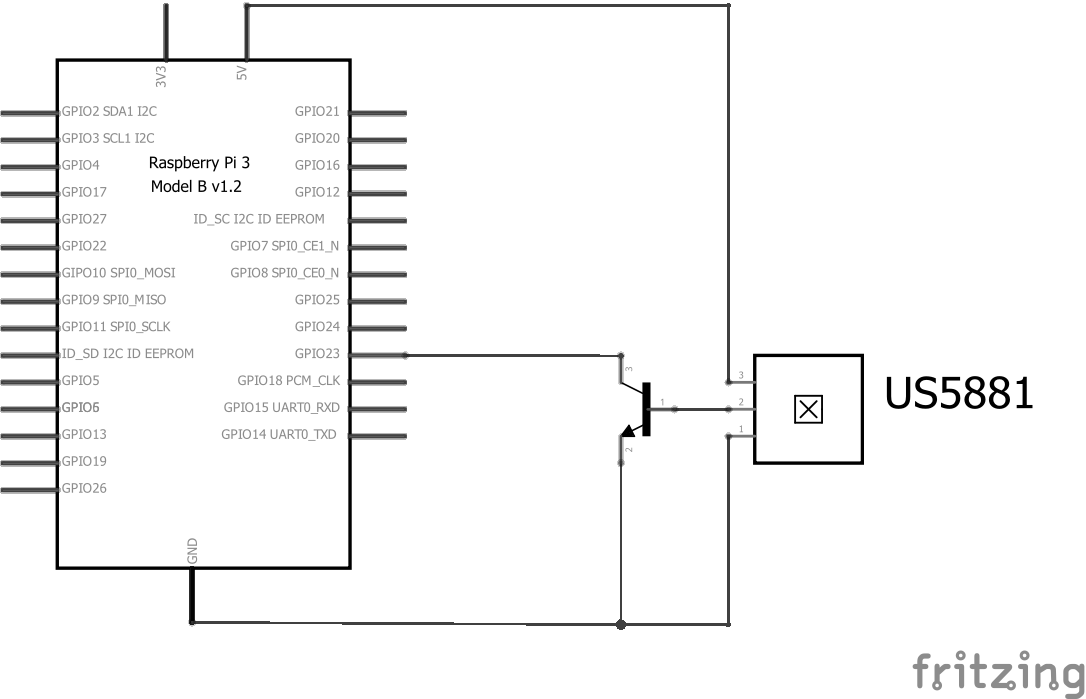
\includegraphics[scale=0.4]{images/circspeeddet.png}}
	%	\caption{Circuit Schematic Diagram: Motor Speed Detection}
	%	\label{circhall}
	%\end{figure} \newline  \noindent
	%This circuit does not measure the instantaneous rotational speed of the motor. Instead it measures the average speed. By using more magnets, and a smaller time-frame, the speed measured becomes closer to an instantaneous speed. The advantage of using this circuit is that it is simple to set up and use, other speed detection circuits require the use of lasers and photodiodes/phototransistors, or dc dynamos and analogue to digital converters. However, the main downside lies in having to attach magnets at regular intervals to the rotating cylinder, which will have to be done accurately. Another downside is the range of the hall effect sensor. The sensor must be within 10mm of the magnet for it to be able recognise it. \newline \newline \noindent
	%Light Sensor
	%The rotational speed of the motor was measured using a light-gate type set up. An IR-LED and IR-phototransistor were set up near the inner cylinder. A metal trip was attached to the cylinder such that it broke the light beam between the LED and the phototransistor. The transistor was set up as a switch such that when light was allowed to fall onto the transistor, a complete circuit was made between GPIO23 (pulled high by the build in resistor) and ground on the Raspberry pi, thus a low value is read. When the beam is broken, this circuit breaks too, causing the value of GPIO23 to go high. On the software side, this value change can be detected and the timing of which can be used to calculate the speed. \newline
	%Dynamo
	The speed of the motor was gauged using a second motor acting as a dynamo (see Figure \ref{circspeeddet} for a schematic of the electronic circuit). The dynamo motor was linked to the first motor by a belt and pulley system. The dynamo motor produces a voltage proportional to the speed it is spun at. This voltage was amplified using an operational amplifier circuit by a factor of ten and read in using an ADC (MCP3008). This was calibrated by setting the potentiometer to different values and recording the voltage produced by the dynamo. Then the speed at these known potentiometer values was found using a tachometer (SERNO). Thus the speed as a function of the dynamo voltage can be calculated. \br
	%\begin{figure}[!htb]
	%	\centering
	%	\fbox{
\includegraphics[scale=0.4]{images/blank.png}}
	%	\caption{Circuit Schematic Diagram: Motor Speed Detection}
	%	\label{circspeeddet}
	%\end{figure}
	There is also a provision for being able to detect the current supplied to the motor. This is achieved using a Hall Effect sensor and inductor pakcage (ACS712). This uses a Hall Effect sensor to detect the size of the magnetic field generated by the current passing through the inductor, producing a voltage proportional to the magnitude of the current. This signal is passed through an op-amp (LM358) to bring it to a suitable level for the ADC to read it.
	

	\subsection{\textit{Motor Speed Control}} % last edited 7/3/2017
	The speed of the motor is sent from the Raspberry Pi as a digital serial signal (using the SPI protocol) to a digital potentiometer (MCP4131), a device which can electronically adjust the resistance between its pins. Within the potentiometer:\(R_{AW}\) is the resistance between terminal Aand the wiper pin, and \(R_{WB}\) is the resistance between the wiper and terminal B. The data sent to the potentiometer determines the values of \(R_{AW}\) and \(R_{WB}\), which will total a constant value: \(R_{pot} = 10,000\ \Omega \). The digital potentiometer is used in a voltage divider configuration, which allows the voltage in a parallel circuit to be controlled. When the resistance is changed to a new value, the voltage across the motor will change according to Equation \ref{eqnvoldiv}. Resistor \(R_2\) is used to set the minimum output voltage. At \(R_2 = 0\ \Omega\), the output would vary between 0v and 5v. While this would also be useful, it limits the resolution of the potentiometer as teh bottom volt of this range will not be able to sufficiently power the motor. To bring this minimum up (and thus be able to utilise more of the potentiometer) \(R_2\) is set at \(3000\ \Omega \). The digital potentiometer can only handle voltages up to 5v across its terminals, an amplifier (gain = 2.1) is used to boost the voltage range from 1.2v to 5v up to 2.52v to 10.5v. A transistor (BD243C) is used to boost the current output from the amplifier, which can only supply around 20mA. The Transistor boosts this up to 2A (assuming a conservative gain of hFE = 100).
	\begin{equation}
		V_{out} = V_{in}\times \frac{R_2 + R_{WB}}{R_2 + R_{pot}}
		\label{eqnvoldiv}
	\end{equation}\newline
	\begin{equation}
		V_{min} = V_{in}\times \frac{R_2}{R_2 + R_{pot}}
		\label{eqnminvol}
	\end{equation}\newline
	\begin{equation}
		V_{max} = V_{in}\times \frac{R_2 + R_{pot}}{R_2 + R_{pot}} = V_{in}
		\label{eqnmaxvol}
	\end{equation}\newline \noindent
	The Raspberry Pi sets the motor speed by setting the resistance in the digital potentiometer. The Pi sends a 7-bit digital signal to the pot, indicating the resistance desired. Within the potentiometer is a network of resistors, and this number will determine the path the circuit takes through the circuit, the higher the number, the higher the resistance between the A terminal and the wiper, \(R_{AW}\). When this increases, the voltage across the bottom resistor will decrease and the voltage across the motor will mirror this. Similarly, when \(R_{AW}\) decreases, the voltage in the bottom half of the divider will increase and so will the voltage across the motor. The resistors included in addition to the digital potentiometer set the minimum and maximum values for the voltage across the motor, the minimum voltage is where the wiper resistance is essentially zero, so Equation \ref{eqnvoldiv} becomes Equation \ref{eqnminvol}. For maximum voltage, the wiper is set as high as possible (\(R_{WB} = R_{pot}\)) and Equation \ref{eqnvoldiv} becomes Equation \ref{eqnmaxvol}. \newline
	%\begin{figure}[!htb]
	%	\centering
	%	\fbox{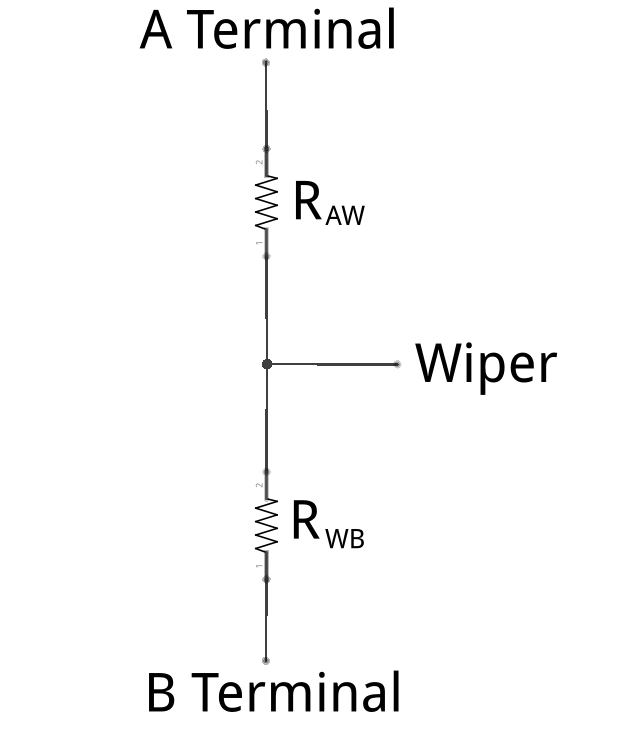
\includegraphics[scale=0.2]{images/circdigpotclose.png}}
	%	\caption{Circuit Schematic Diagram: Digital Potentiometer Detail}
	%	\label{circdigpotclose}
	%\end{figure} \newline  \noindent
	%\begin{figure}[!htb]
	%	\centering
	%	\fbox{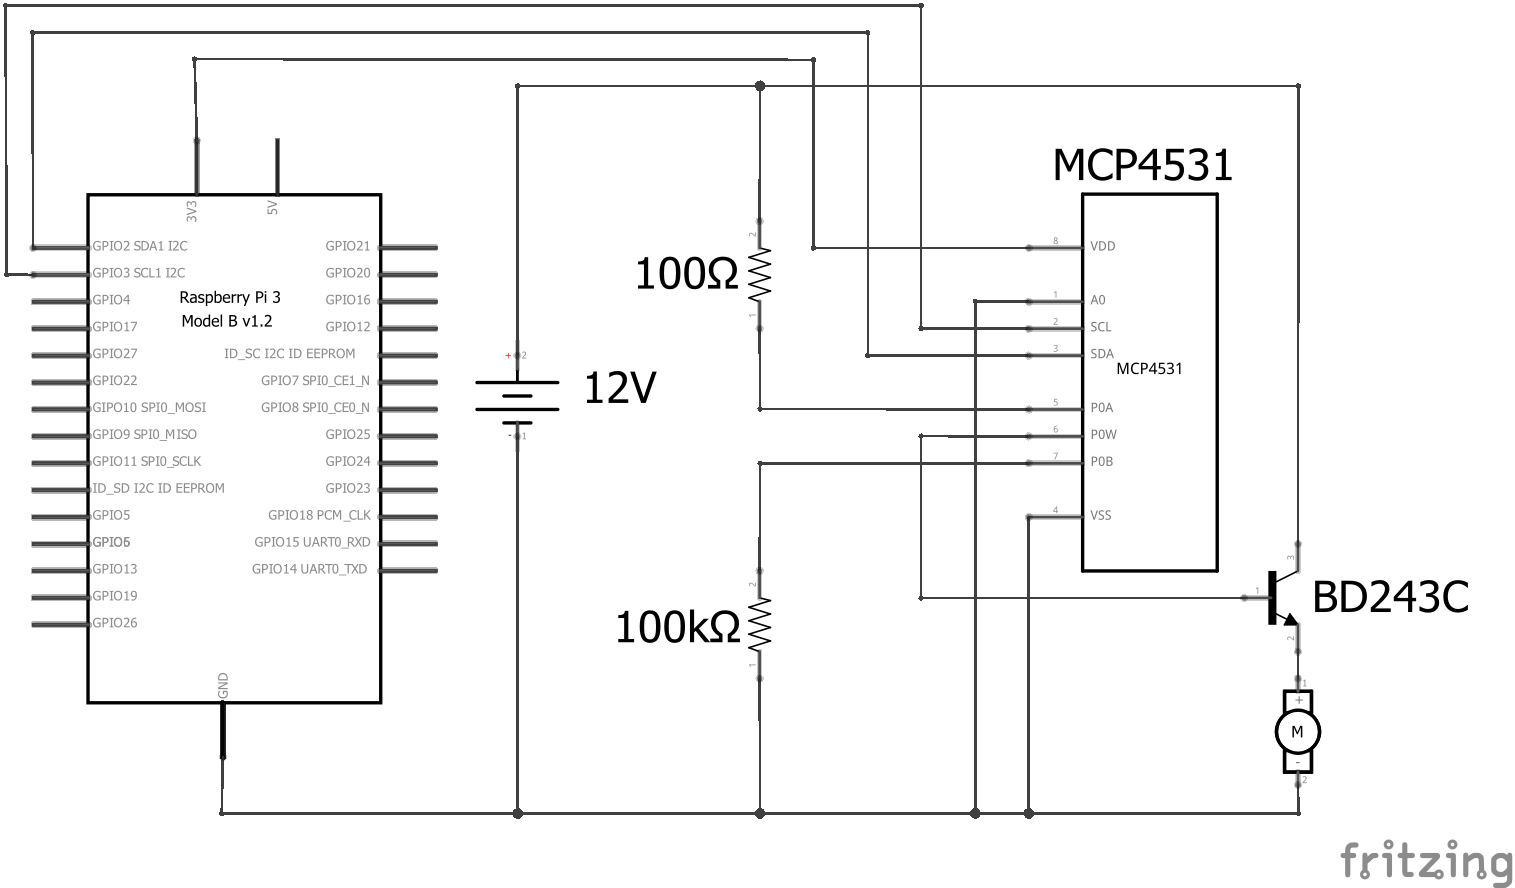
\includegraphics[width=\textwidth]{images/circspeedcontr.png}}
	%	\caption{Circuit Schematic Diagram: Motor Speed Control ADD RESISTOR NAMES}
	%	\label{circspeedcontr}
	%\end{figure} \newline  \noindent


	%\subsection{\textit{PEND Input Processing}}



	\section{Software} % Re do section
	To manage the hardware connected to the device, software was written in Python, using software packages from its extensive (community driven) online repositories. The object-oriented nature of the language was fully utilised in order to create class-based code that was easy to read so that another person wanting to use the software would be able to understand how it works. In addition, the classes make it easy to add additional functionality to the experiment (adding other sensors or motors to increase the scope of the experiment). The software was composed of five main classes: exp\_run.py, control.py, motor.py, dig\_pot.py, and adc.py. \newline \newline \noindent
	A master script controls all of the classes and controls the overall flow. It looks for run information and checks whether there are runs to be done. Data defining the parameters of the experimental runs is contained in a comma separated value (CSV) file. This information is read in by the \(exp\_run\) class, which uses this to run the motor at the correct speed using the \(motor\), \(dig\_pot\), and \(control\) classes. The PEND sensor input is read in using the \(adc\) class. See Figure \ref{codemap} for a diagram of communication between the classes. \newline 
	\begin{figure}[!htb]
		\centering
		\fbox{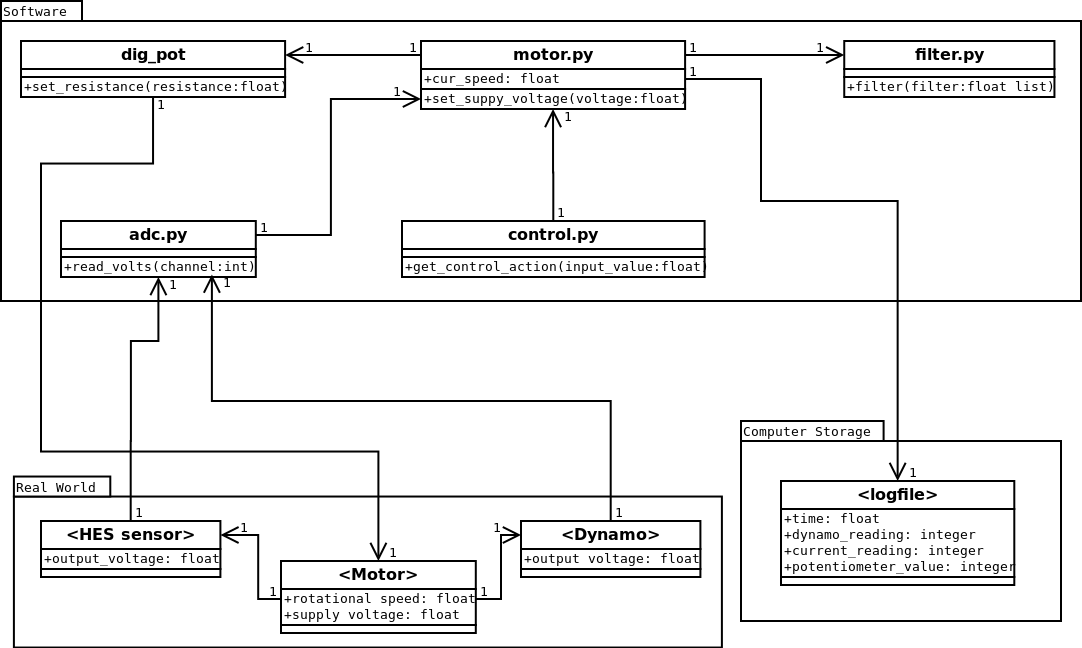
\includegraphics[scale=0.3]{images/codemap.png}}
		\caption{Code Map Diagram (RE DO RE DO RE DO)}
		\label{codemap}
	\end{figure}
	EXPLAIN THE DIFFERENT SCRIPTS AND CLASSES



	\section{Design Evaluation}
	%The project can be split into different sections; design, development, and evaluation. In the design phase the overarching goal of the system was decided, including the scope and acceptable limitations. During the development phase prototypes of the system were created and tested against the design specification, altering and improving as necessary. Finally, the evaluation phase saw the use of a completed version of the control system in a rheology experiment, benchmarked against the results of standard lab equipment to gauge the utility of the bespoke apparatus.
	
	\subsection{Voltage Control} % Add figure
	The DC motor used in the experiment was able to accept an electrical supply of variable voltage; between 4.5v and 15v. Due to the relatively low speeds required by the shear cell, it was decided that the motor would be controlled in a shifted voltage range, between 2.5v and 10.5v. 
The low end of that range being 2v less than the motor's minimum voltage was a design artifact, but was later found to adequately power the motor at low speeds. %%%%%%<----------------------------------------------------------------------------------------------------------------------------------------------------------------------------------------
The circuit was deemed to be satisfactory if it could achieve quick and reliable control over the motor's supply voltage. This was tested by using a script to automatically vary the controlled voltage, and a voltmeter placed in parallel across the motor. The values were recorded for selected values (between 0 and 127, in steps of 16) of the potentiometer, resulting in a correlation between the potentiometer value and the voltage supplied to the motor. The voltage varied linearly with potentiometer value (see figure \ref{figvoltvval}) between the desired minimum and maximum thus proving the circuit to be satisfactory.
	\begin{figure}[!htb]
		\centering
		\fbox{\includegraphics[scale=0.3]{figures/figvoltvval.png}}
		\caption{Motor Voltage Supply vs. Potentiometer Value}
		\label{figvoltvval}
	\end{figure} \newline  \noindent

	\subsection{Speed Measurement}
	The rotational speed of the motor needed to be measured accurately and quickly, to be able to calculate the viscosity, and to ensure high enough sample rate that the jamming phenomenon can be seen. This was achieved by using a second motor as a dynamo, linked to the controlled motor via a belt. The dynamo will be spun and generate a voltage proportional to the rate at which it is spun, similar to the speedometer in a car [CITE?]. The magnitude of the voltage can be read in using an ADC by the Raspberry Pi (up to 200,000 samples per second). Accuracy of the set-up was tested using a slow-motion camera to film the rotation and gauge the actual rotational speed, compared with the value obtained using the dynamo.
	\begin{figure}[!htb]
		\centering
		\fbox{\includegraphics[scale=0.3]{figures/figspeedvval.png}}
		\caption{Read Speed and Actual Speed vs Potentiometer Value}
		\label{figdynocheck}
	\end{figure} \newline  \noindent
	Figure \ref{figdynocheck} shows how the actual speed of the motor and the read value compare. It can be seen that the two values correspond well. This uses little of the computing power of the Raspberry Pi as all it has to do to obtain the rotational rate is read a value in from an ADC and perform a simple multiplication; thus this can be performed accurately and at high frequency - well suited to the required purposes.\br
	In order to confirm the accuracy of readings, several videos were taken (at 120fps). The speed was set at a constant value for 10 second periods before lowering during filming, allowing the speed at different potentiometer values to be recorded. A mark was made on the rotating cylinder and as this mark passed a certain point, a counter was increased. After the 10 second period, the counter total represented the number of rotations in 10 seconds, the speed in RPM can be calculated by multiplying by 6. This was repeated several times with several different recordings to ensure the resulting correlation was correct. \br
	To decypher whether this method was quick enough, the motor was set at a single speed, and the speed was recorded at different set intervals. The standard deviation of the resulting speed curves was taken for each interval. Ideally, these should all be the same and equal to zero. %Is this feasible? or just some quality bullshit?
	
	
	
	\subsection{Speed Calibration} % Rework
	There are several parameters that need to be calculated before the motor can be used in the rheometer. The torque and efficiency characteristic curves of the motor need to be calculated (OR FOUND??). To find this, the digital potentiometer was set to 0 and initial readings of the speed and voltage were taken. Then the value was incremented, the motor speed and voltage were recorded. This was done for every possible value for the digital potentiometer. Using the recorded information, a relationship was found between efficiency and speed. This allows the torque to be calculated using only the electrical power input to the motor, and the rotational speed of the motor (see Equation \ref{eqntorque}).
	\begin{equation}
	\tau = \frac{I \times V \times \eta}{\omega}
	\label{eqntorque}
	\end{equation}
	
	\subsection{Current Sensor}
	To sense the current drawn by the motor, a hall effect sensor is used. A hall effect is able to produce a voltage proportional to the strength of a magnetic field, a magnetic field which can be produced by running a current through a coil with a magnetically permeable core. The sensor package contains both the coil and the hall effect sensor such that when a current is passed between the sensor pins, a voltage proportional to this current is produced accross the output pins. The sensor used is the ACS712 package using a 5v supply from the Raspberry Pi. The normal output (at zero amps sensed) is half of the supply voltage. The direction of the current will determine whether the current will increase (reverse direction) or decrease (forward direction) this voltage. \br
	The current draw by the motor will only ever be in a single direction, so the direction information is not necessary. To increase the resolution, 2.5v is subtracted from the signal before it is amplified by 10 and fed into the ADC (channel \#1). \br
	The sensor was calibrated by reading in from the sensor and comparing this value with the actual current reading obtained using a standard lab multimeter, repeating this at different voltages (thus also different rotational speeds and different currents). \br
	[RESULTS AND SUCH]
	
	\subsection{Motor Torque Calibration (NECESSARY??)}
	The torque output from the motor with respect to the voltage applied to the motor must be known to be able to calculate the rheology of the liquid in the couette cell. There are two torques output from the motor: the load torque, and the shaft torque. The former is the torque imposed upon the load, and the latter is the torque imposed upon the motor's shaft. \newline \newline \noindent 
	There are limits upon the motor's output, at high enough torque, the rotational speed will reach zero. This torque value is the \textit{stall torque (\(\tau_s\))} and represents the maximum value of torque able to be output by the motor. The second limit is where the motor has no load imposed upon it. The torque here is the no-load torque (equal to the shaft torque). The rotational speed here is the greatest possible value (for a particular voltage) and can be used to calculate the no-load torque and thus the shaft torque. \newline \newline \noindent
	By recording the voltage and current through the motor, the power input to the motor can be calculated. Using the electrical power and the efficiency, the mechanical power output and the torque output can also be calculated. The speeds at different loadings were recorded, giving the torque in terms of the voltage/current (power). (REWORD?)


%=====------++++++=====------++++++=====------++++++=====------++++++=====------++++++=====------++++++=====------++++++=====------++++++=====------++++++=====------++++++=====------++++++=====------++++++=====------++++++=====------++++++=====------++++++=====------++++++

	\chapter*{Conclusions}
	\addcontentsline{toc}{chapter}{Conclusions}
	\def\achapter{Conclusions}
	%Summarise findings and inferences mentioned in the core of the report. Try to be as brief as possible, with concise statements. Include recommendations, where appropriate. 
	
%=====------++++++=====------++++++=====------++++++=====------++++++=====------++++++=====------++++++=====------++++++=====------++++++=====------++++++=====------++++++=====------++++++=====------++++++=====------++++++=====------++++++=====------++++++=====------++++++


	\chapter*{Review}
	\addcontentsline{toc}{chapter}{Review}
	\def\achapter{Review}
	%Relate this section to the learning objectives in the introduction. Report what you have learnt about the organisation and about yourself. Mention your achievements, what you have learnt, skills you have acquired or improved. This might be technical or "soft" skills. Try to relate this to what you have learned in your coursework at University and what skills you will take forward to your first full time professional post.
	

%=====------++++++=====------++++++=====------++++++=====------++++++=====------++++++=====------++++++=====------++++++=====------++++++=====------++++++=====------++++++=====------++++++=====------++++++=====------++++++=====------++++++=====------++++++=====------++++++

	\chapter*{Nomenclature}
	\addcontentsline{toc}{chapter}{Nomenclature}
	\def\achapter{Nomenclature}
	%List all the symbols in alphabetical order, with Greek symbols at the end.
	\begin{center}
		\begin{tabular}{|c|l|}
			\hline
			\rule{1cm}{0pt}\textbf{Symbol}\rule{1cm}{0pt} & \rule{4cm}{0pt}\textbf{Description}\rule{4cm}{0pt} \\
			\hline
			\( R_{1} \) & Voltage divider resistor 1 resistance, ohms \\
			\hline
			\( R_{2} \) & Voltage divider resistor 2 resistance, ohms \\
			\hline
			\( R_{AW} \) & Potentiometer resistance between the wiper and the "A" terminal, ohms \\
			\hline
			\( R_{pot} \) & Potentiometer resistance, ohms \\
			\hline
			\( R_{WB} \) & Potentiometer resistance between the wiper and the "B" terminal, ohms \\
			\hline
			\( V_{out} \) & Voltage output from the potentiometer voltage divider, volts\\
			\hline
			\( V_{in} \) & Voltage input to the potentiometer voltage divider, volts\\
			\hline
			& \\
			\hline
			& \\
			\hline
			& \\
			\hline
			& \\
			\hline
			& \\
			\hline
			\( \mu \) & Viscosity, in Pa.s\\
			\hline
			\( \sigma \) & Shear Stress, in Pa\\
			\hline
		\end{tabular}
	\end{center}
	
	%Main Bibliography
	\newpage
	\addcontentsline{toc}{chapter}{Bibliography}
	\def\achapter{Bibliography}
	\bibliography{biblio}
	\bibliographystyle{unsrt}
	%\bibliographystyle{apalike}

%Appendix


\appendix


\chapter*{Appendices}
\addcontentsline{toc}{chapter}{Appendices}
\def\achapter{Appendices}
\pagenumbering{alph}
\setcounter{page}{1}
\setcounter{section}{1}
\section{1 - Further Information}
\subsection{A -  Programming Languages}
Programming languages come in many forms. High level languages (like C, Java, C\#, Python) are abstracted from the binary in which it will be eventually stored. High level languages consist of a natural-like language which is converted by a "compiler" or "interpreter" into machine code, understandable by the processor \cite{proglanghighlow}.\newline \newline  \noindent
\noindent
An example of a high level language (Python):
\begin{verbatim}
                    from time import time()

                    alarm_time = 2147483647

                    while (time() < alarm_time):
                         pass

                    print("Alert!")
\end{verbatim}
An example of a machine code (in hexadecimal)\cite{proglangmachex}:
\begin{verbatim}
                    0x 60 00 00 80
                    0x A4 00 00 00
                    0x 60 01 00 84
                    0x A4 01 01 00
                    0x 60 02 00 00
                    0x 60 03 00 04
                    0x 60 04 00 00
                    0x 60 05 00 01
                    0x 08 00 00 02
                    0x 20 00 00 03
                    0x 20 04 04 05
                    0x 11 20 04 01
\end{verbatim}
	From the above it can be seen that high level languages, while not strictly English, are far easier to read than machine code. Machine code will take multiple instructions to achieve the same thing that could be done in a single line in a high level language, thus a high level instruction needs to be converted into multiple machine level instructions for the processor to understand it. There are different ways of doing this, leading to diversity in the types of high level languages. \hi (MISSING LINK) \nohi. Object Oriented Programming Languages (OOPLs) deal with data in terms of "objects"\cite{proglangwhatisoopl}. An object is, like the name suggest, something. This something has properties, and can have things done to it. In the above Python example, "alarm\_time" is a number object, and it is being assigned a value. A "method" is a way of doing something in the program. In the above, the "time()" method is used to get the current time (in number of seconds since 1 January 1970). The advantage of OOPLs lies in the ability to collect objects and methods together in a class. The "time" class above contains a lot of methods which can be used by the programmer, in the example the "time.time()" method is called from the class. The programmer can therefore define a set of methods for dealing with some data in a certain way in a class, and then create multiple instances of this class with different starting data to make use of different starting data. For example, a "sphere" class could be written, with methods which provide the sphere's surface area and volume, given the sphere's diameter. Then a program could be written to create three sphere class instances, each with different diameters and then the areas and volumes could be calculate simply when needed. This creates tidy programs, which are easier to understand and reduces the amount of redundant code that needs to be written.\newline \newline  \noindent
	Another, less common, type of programming language is the procedural language. This language is simply one instruction following another\cite{proglangwhatisoopl}. The procedural program starts at the start and continues down the list of instructions until it finishes. This language requires writing out the same code multiple times to achieve the same effect as an OOPL, which is a reason for its reduced popularity.\newline \newline  \noindent
	As previously mentioned, code written in a programming language is usually compiled before it is run. However, some languages do not need to be compiled before being run. These languages are called "interpreted" languages and they are "compiled" line by line when you run them \cite{proglanginterp}. Since interpreted languages do not need to be compiled (and so software developers do not have to wait for the compilation step to complete before testing) they are preferred for developing software. However, they tend to run slower than compiled programs for the same reason.\newline \newline  \noindent
	To conclude this section,  programming languages are varied and have different advantages and disadvantages. The correct programming language must be chosen for the correct situation.\newline \newline  \noindent

\section{2 - Design Process Discussion}
\subsection{A - Voltage Control}
\subsection{B - Measuring Speed}
The rotational speed of the motor needed to be able to be measured both accurately and frequently (at least 40 times every second - data gathered at most every 25ms). The final design used to meet this specification made use of a dynamo linked up to the motor to gauge the speed of rotation (see Description of Work, page \pageref{chap:dow}). Discussed here are two methods which were considered for use, but were not able to meet the specification.\br 
The first design prototyped for use as a speed sensor was a Hall Effect Sensor coupled with a magnet. The set up was such that every rotation, the magnet would trigger the hall effect sensor and the \rpi would see this trigger as a new revolution. By recording the time between revolution triggers, it would be possible to calculate the rotational speed of the motor. The design was tested for compliance by altering the potentiometer value, thus varying the supply voltage and rotational speed of the motor. The rotations were read in by the sensor, the time of each detection was logged, along with a running log of the speed (recorded every 0.1s). The potentiometer value was held for 10 seconds to allow any dynamic responses in the speed to settle away. If there are any dynamic elements to the motor's speed as a result of a change in voltage, it would show in the results as an altered initial value after a change, which quickly settles to a constant value after  a period of time. The data recorded was evaluated using a histogram plot of the interval times between detected rotations, and a line plot of the measured speed (using both methods) against potentiometer value. \newline \newline \noindent
The histogram should be a single straight line indicating no variation in interval time. If there is found to be small variation in the time, this could be small variation in the supply voltage due to changes in the electrical mains - this would be the main disturbance the control system is working to defend against. Small variation can also be explained away as a leftover between potentiometer value changes with little to no impact on the overall data. Large variation in interval time indicates that something is not right, either with the circuit or the software. It is more likely to be a software error or a limitation of the Raspberry Pi itself rather than a circuit design issue due to the digital nature of the sensor - it can only be on or off. It is unlikely that the sensor is giving a false positive part way through a revolution, or a false negative. \newline \newline \noindent
The line graph of speed against potentiometer value should display two lines which are almost exact copies of each other and are easy to describe lines, preferably linear.\br
	\begin{figure}[!htb]
		\centering
		\fbox{
		\begin{subfigure}[t]{0.45\textwidth}
			\centering
			\includegraphics[scale=0.35]{figures/figsenshisto.png}
			\caption{Histogram Plot of \newline Sensor Input Interval Time (WHICH SETTINGS GIVES THIS?)}
			\label{figsenshisto}
		\end{subfigure}
		\begin{subfigure}[t]{0.45\textwidth}
			\centering
			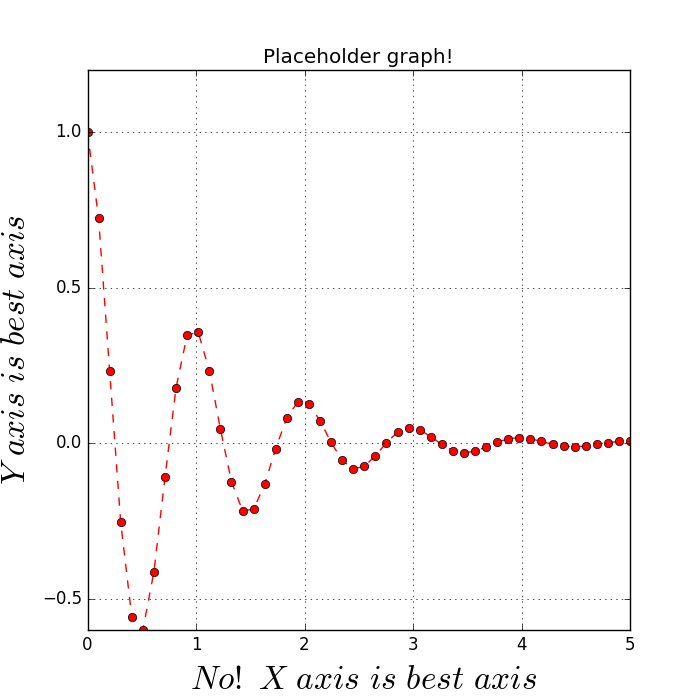
\includegraphics[scale=0.35]{figures/placeholderfig.png}
			\caption{Motor Rotational Speed vs. \newline Digital Potentiometer Value}
			\label{figspeedvval}
		\end{subfigure}
		}
		\label{fig2speeds}
		\caption{Speed Calibration Results}
	\end{figure} \newline  \noindent
	The histogram shows that the intervals are not a constant value (Figure \ref{figsenshisto}). The interval variance is not negligible, and by inspecting the raw data, it was found that the sensor was failing to record some rotations (especially noticable at low speeds). After multiple attempts (with different magnet position, different strengths of magnets) the sensor could not be found to work accurately enough. Perhaps there was a fault in the software, perhaps the \rpi was not able to process the information fast enough, or perhaps the hall effect sensor was simply not able to cope with the repeated switching. The second is highly unlikely; the CPU load on the \rpi was checked on several occasions and was found to only be around 3\% of maximum - the Pi was not at all struggling to run the script.\br
	The speed comparison was [RESULTS2] (Figure \ref{figspeedvval}) therefore this design meets the specified requirements and is suitable for use.
\section{3 - Alternative Designs}
\subsection{A - }
%Appendix Bibliography

\end{document}